\documentclass[12pt]{amsart}

\usepackage{a4wide}

\usepackage{fancyhdr}
\pagestyle{fancy}
\lhead{}
\chead{}
\rhead{}
\lfoot{}
\cfoot{\today}
\rfoot{\thepage}

\usepackage{algorithm2e}
\usepackage{graphicx}
\usepackage[parfill]{parskip}
\usepackage{appendix}
\usepackage{amsmath}
\usepackage{multicol}

\renewcommand{\labelitemi}{-}
\renewcommand{\labelitemii}{-}
\renewcommand{\thefootnote}{\roman{footnote}}

\setcounter{secnumdepth}{10}
\setcounter{tocdepth}{3}

\title{Trader Game}
\author{Ethel Bardsley, Joseph Slade and Thomas Wood}

\begin{document}

\maketitle

\section{Introduction}
  % Brief rundown of the spec
The purpose of this exercise was to gain experience with web programming, 
with running server and client side testing,  and with use of a database, 
all for the purpose of making a multi user program. Specifically,  
this program was a space trading game.  Whilst we stuck with the essence
of this program,  we made a few changes in areas in which we felt we could
improve the core game.
\section{Concept}
  % Brief explanation of the game
  The primary idea of the game was to be a trading game,  as in the original 
spec. We felt that this was a good model for a game,  but we decided to make 
some key changes.  
  \begin{itemize}
    \item Cross-Platform\\
      A cross-platform game has several advantages. It can be played by players
      on any machine, increasing potential audience by a reasonable factor. It
      also allows for testing and development to be done on any platform, which
      certainly makes development easier.  

    \item Multiple maps with a means of teleporting between them\\
      Multiple maps with single points of access allow interesting modifications
      to core gameplay to be made in certain zones.  Because separate maps form
      distinct environments,  they can justifiably (in an in-game sense) have
      different enemies,  different items in their shops,  and even allow certain
      things that could not be implemented on a universal scale,  such as free
      for all PvP (see next section), or co-operative PvE (see next section).
      Although we did not have this implemented at the time this report was
      written, we would like to have a working prototype of it for the presentation.

    \item PvE and PvP\footnote{Player versus Environment, Player versus Player}
    interaction\\
      The main selling point of all multiplayer games is the fact that the player can
      interact with others.  Player versus Player (PvP) interaction in any game generally 
      consists of either combat or trade.  We chose to implement both,  and players can
      attack each other as they wish.  There is currently nothing to gain
      from combat,  except for preventing other players from logging their character
      in once dead which has its appeal to certain players.  Players cannot trade
      directly, but the game economy is a dynamic,  and one player purchasing all
      of a resource will cause a shortage of that resource for a period of time.

    \item A dynamic economy where the value of an item is related to its
    rarity\\
      To provide some concept of a goal,  and as an alternative to destroying
      other people's characters,  players can buy and sell resources.  The system 
      is not zero sum\footnote{There is not a fixed amount of gold in the economy}, and
      so players have the opportunity to make money. To prevent this aspect of the game
      being about more than making round trips between two points where there 
      is a fixed discrepancy between item values,  item stocks and values fluctuate over time,
      modified by various factors,  such as the map the shop is on,  the amount of stock
      held at a time,  and any other reasonable thing we can think of.


  \end{itemize}

\section{Program Design}
  \subsection{Renderer}
    \subsubsection{Choice of Technology}
      \begin{flushleft}
        There are a variety of technologies for browser-based rendering. The
        most obvious is Adobe Flash, as well Microsoft's Silverlight. However,
        while these are powerful tools with a wide selection of libraries and
        well-trodden paths for development, neither are universally cross
        platform, and Silverlight is not supported by the version of Firefox
        on the test machines.

        For handling the rendering with just HTML and Javascript, one method is
        to render by manipulating the DOM\footnote{Document Object Model}, and
        there are a few libraries for writing renderers using this method.
        However, DOM manipulation can suffer performance issues, particularly
        where there are many elements being drawn.

        Canvas is a relatively new technology, introduced with HTML5. It allows
        for procedurally drawing directly to an image with Javascript, and is
        supported by Gecko, WebKit (including mobile versions) and, from version
        9, Internet Explorer. There aren't many libraries available for it, and
        those that are aren't mature or well documented. However, canvas itself
        has sufficient framework for 2D sprite drawing.
      \end{flushleft}

    \subsubsection{Implementation}
      \begin{flushleft}
        The render initialises by setting up the canvas element and render
        context, loading map data from the server, using that to generate a
        background image and place any scenery sprites (e.g. shops). It then
        centers the view, adds an input handler, before starting the render
        loop.

        The field in the background is procedurally generated, being a
        different image each time the page is loaded. Pixels are a random
        colour, weighted toward being a light green. Originally, we tried to have
        each pixel in the map generated uniquely, but this was too CPU
        intensive, causing the page to hang, or even crash. To remedy this,
        it instead generates a set of temporary smaller canvas tiles and uses
        those to build the larger background, which is considerably more
        performant.

        Sprite animation currently supports two actions, \verb/stand/ and
        \verb/walk/, although it could be easily extended as needed. Each
        action has a number of sprites associated with it, which are simply
        stepped through, one per redraw, moving the sprite across the screen if
        necessary. Because of this simplicity, attacking motions must
        happen independently in their own render queue to prevent the main
        actor sprite from disappearing.
      \end{flushleft}

  \subsection{User Interface}
    \begin{flushleft}
      The UI is set out with the gameboard at the centre of the page, with
      all information displayed to the user on either side
      of the board. This balances the display aesthetically and provides a clean intuitive
interface for the user. Given more time, we would have further improved the design of the
webpage.

It was a design choice to simplify the registration process of the game to the extent that the only
information required is the user's name. This simplification reduces the steps needed to start playing,
which will hopefully draw more users in. The flipside of this is that automated registration is trivial,
so the game may be open to abuse, particularly as all players can send and view chat.
\end{flushleft}

\begin{figure}[h]
\begin{center}
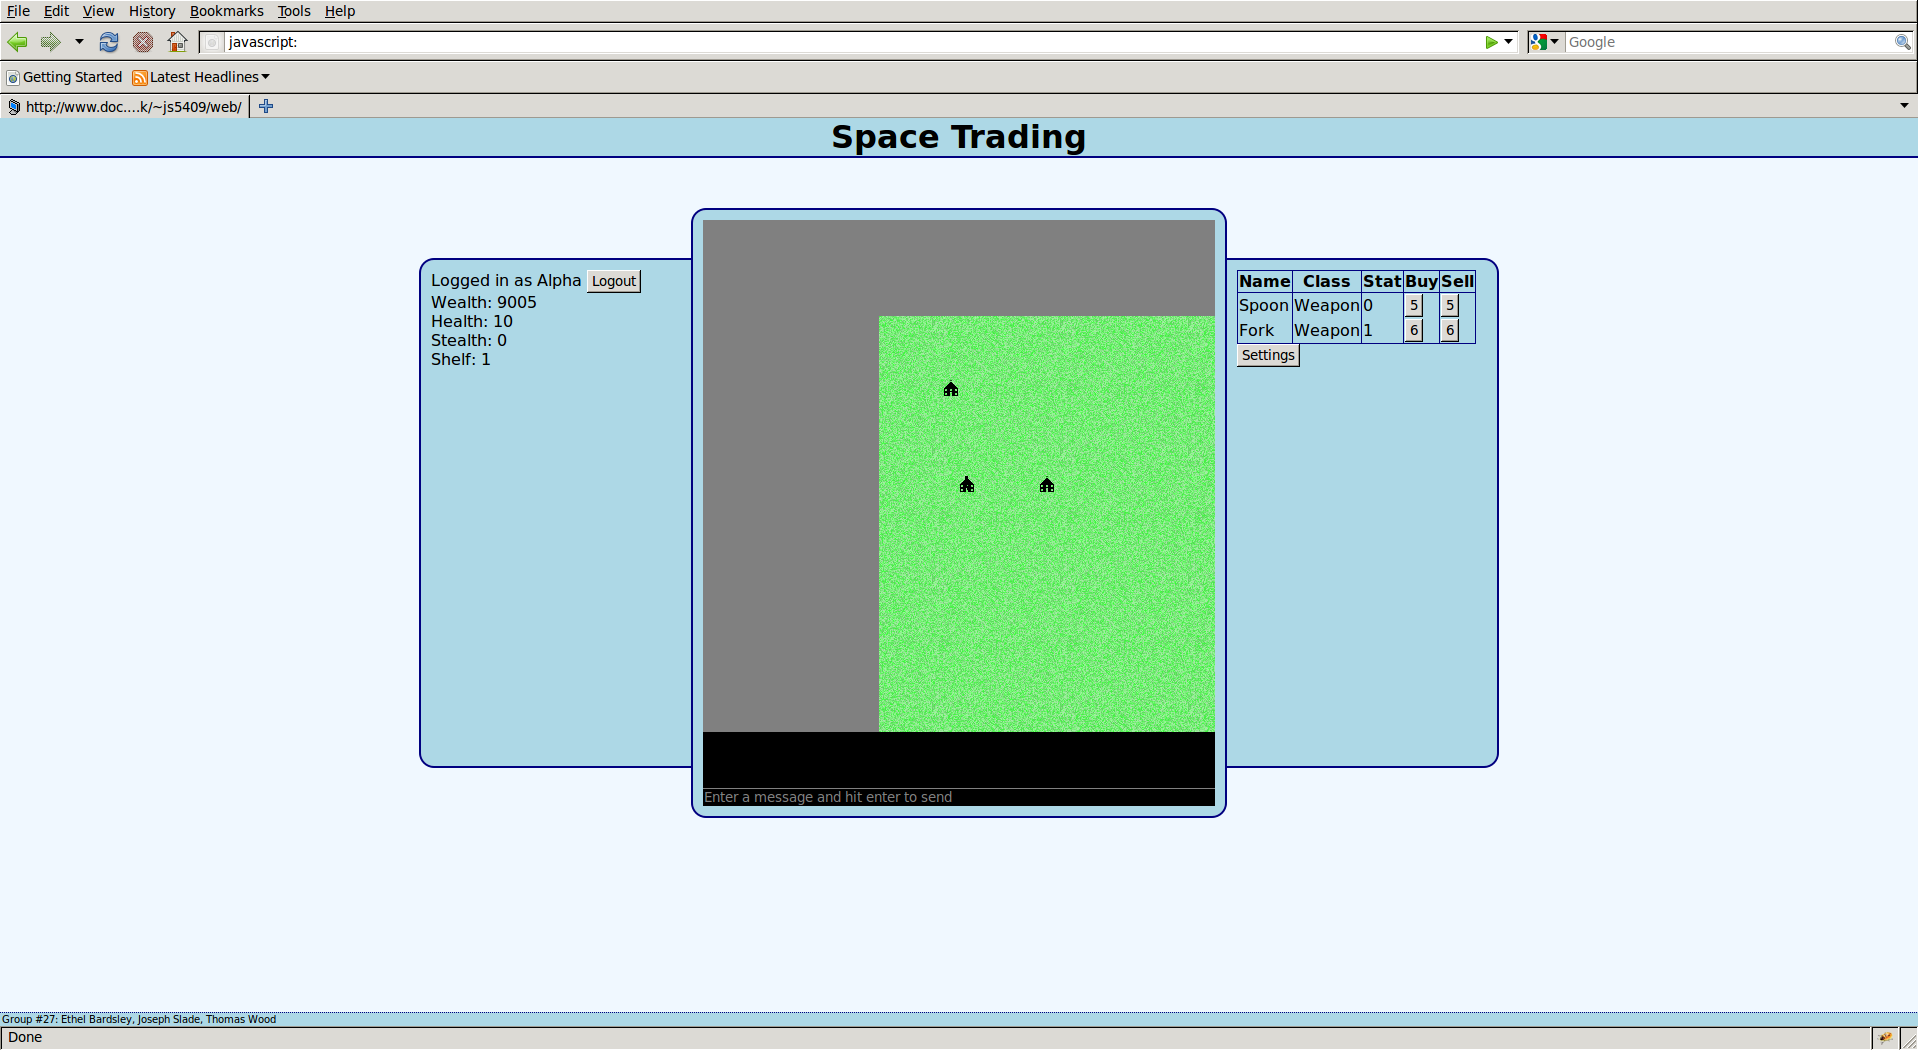
\includegraphics[width = 0.95\textwidth]{screeny}
\caption{Screenshot of the game interface, the green is the map, the grey is off map, the panels to either side of the canvas contain the additional controls and game state information, the black panel below the map displays notifications and chat messages}
\end{center}
\end{figure}

  \subsection{Network}
    \begin{flushleft}
      The frontend makes extensive use of the XMLHttpRequest interface provided 
      by the browser. This interface permits additional HTTP requests to be made 
      to the server by the client-side JavaScript to request that an action be 
      recorded in the database, or to receive more data.

      The client to server data encoding is the same as a standard HTML form 
      would be transmitted as, namely the 
      \verb|application/x-www-form-urlencoded| MIME-type. This is reasonably 
      simple to construct with JavaScript, with each field name and value
      string being URL-escaped then concatenated into a string with \verb|=| 
      separating the fields from the values, and \verb|&| being used to separate 
      each individual field.\footnote{See also: W3C HTML 4.01 Specification Section 
      17.13.4} This format is advantageous for receipt on the server-side as PHP 
      automatically parses requests made in this format and makes them available
      to the program.

      The server to client data is encoded using JSON\footnote{JavaScript Object 
      Notation}. This format is advantageous as a transfer format as it 
      concisely encodes complex data-structures into a reasonably human-readable 
      string. Both PHP and JavaScript provide built-in functions to encode and 
      parse this format, respectively.

      We have also implemented a server-push notifications system using the 
      long-polling of multipart HTTP requests. HTTP is generally limited by the 
      fact that requests can only be made in one direction - a client can only 
      request data from a server, the server cannot arbitrarily open a 
      connection to the client to notify it of an event.
      
      Long-polling is one 
      method to overcome this limitation. Long-polling is when a client makes a 
      request to the server to send it data but if the server has no data to 
      send at the time the request is made, the server holds the connection open 
      until it is ready to send some.
      
      Multipart requests permit multiple distinct responses from the server to 
      the client for an individual request. In standard practice, the content of 
      any previous responses is replaced by the content a new incoming response.

      The combination of long-polling with multipart responses permits 
      server-pushing to be achieved. As an added precaution against underlying 
      connection timeouts, each long-poll request is terminated after 60 seconds 
      and re-initiated.
    \end{flushleft}

  \subsection{Backend}
    \subsubsection{Choice of Technology}
      \begin{flushleft}
      Our choice of server-side technology was decided by a combination of the
      skills the members of the group already had and for the ease of use with
      the department's Apache server. We chose PHP as the backend programming
      language for several reason: there was a minimal setup time
      required to get code to work with the provided server, the
      language transparently deals with many of the complexities of handling
      requests, PHP's syntax is very similar to C's and it promotes a programming style close to
      that used in Java, both languages that the group are familiar with. Finally
      PHP has, built in, a large number of interfaces to external libraries. we made 
      particular use the PDO\footnote{PHP Data Objects} class to interface
      with the PostgresSQL database and the SystemV Semaphore library for
      low-overhead message passing between processes.       
      \end{flushleft}

    \subsubsection{Implementation}
      \begin{flushleft}
        Our code structure aims to meet the MVC\footnote{Model View Controller} 
        pattern of object-oriented programming. To achieve this we opted to use a third 
        party PHP library, the ToroPHP Framework.\footnote{http://www.toroweb.org/, 
        the code is assumed to be freely licenced as all documentation implies so} 
        ToroPHP a small (150 line) class to route requests to appropriate handler 
        (controller) classes.

        We implemented a basic object-relational mapping class to make database 
        requests as straightforward as possible. There exists an abstract 
        DatabaseRecord class that handles the each of the standard 
        CRUD\footnote{Create, Read, Update, Delete} actions for all database 
        access. Each individual table has its own class subclassed from 
        DatabaseRecord, set on each of these classes are the fields that are 
        contained and associated functions, such as the login function on the 
        Player class.

        One of the model classes does not use the PostgresSQL database as a 
        backend. For the backend to the long-polling message notifications we
        are using Unix SystemV Shared Memory and Message Queues. We opted to use 
        these rather than the database to minimise the overheads that would 
        result from continually polling the database. Instead, the 
        implementation of reading from the Message Queue cause the process to
        become blocked until an appropriate message is placed in the queue.
      \end{flushleft}

\section{Conclusion}
  % Wrap up, reiterate all the above in short
  \begin{flushleft}
    While we did not acomplish everything we set out to do, we were for the
    most part successful, and with extra time could have accomplished more. 

    For example, the multiple maps with teleporting feature was not implemented
    by the time the report was written, although the database framework for it
    exists. 

    The economy daemon to alter the number of items available to emulate supply and demand was unimplemented. However it could be done with simple set of SQL  queries.

    The combat provided is highly simplistic, just deducting your `shelf' from
    their health. However, as with maps, the framework is there and is easily
    extended to include item/wealth drops, weapons of different ranges, and so
    on.

    Also, the game is not terribly pretty. This is entirely down to the lack of
    artistic skills on the team. We attempted to make more detailed 32px
    sprites, however they looked worse than the 16px ones.
  \end{flushleft}

\end{document}

